\documentclass[a4paper,12pt]{article}
\usepackage[paperwidth=210mm,paperheight=297mm,left=27mm,right=27mm,top=27mm,bottom=27mm]{geometry}

%%%%%%%%%%%%%%%%%%%%%%%%%%%%%%%%%%%%%%%%%%%%%%%%%%%%%%

\usepackage[onehalfspacing]{setspace}
\usepackage{rotating}
\usepackage{caption}
\usepackage{lscape}
\usepackage{epstopdf}
\usepackage{graphicx}
\usepackage{amsmath}
\usepackage{threeparttable}
\usepackage[utf8]{inputenc}
\usepackage{natbib}

%%\usepackage{float}

\usepackage{bibentry}

\bibliographystyle{apalike}

\usepackage{eurosym}
\usepackage{amssymb}
\usepackage{amsmath}
\usepackage{graphics}

\usepackage{verbatim}
\usepackage{multirow}
\usepackage{floatrow}

		\floatsetup[table]{capposition=top}

\usepackage{float}

\usepackage{longtable}
\usepackage{pdflscape}

\usepackage{comment}
\usepackage[title]{appendix}
\usepackage{placeins}

\usepackage[thinlines]{easytable}


\usepackage{xcolor}
\usepackage{color, colortbl}

	\definecolor{Gray}{gray}{0.9}
	\definecolor{LightCyan}{rgb}{0.88,1,1}

\usepackage{afterpage}

\usepackage[hyphens]{url}


\usepackage[colorlinks,breaklinks=true]{hyperref}

\hypersetup{pdfnewwindow=true}

\hypersetup{
     colorlinks   = true,
     citecolor    = black
}

\hypersetup{linkcolor=blue!75!black}
\hypersetup{urlcolor=blue!75!black}
\hypersetup{filecolor=blue!75!black}
\hypersetup{citecolor=purple}


%%%%%%%%%%%%%%%%%%%%%%%%%%%%%%%%%%%%%%%%%%%%%%%%%%%%%%

\begin{document}

\title{Does domestic demand matter for firms' exports?}
\author{Paulo Soares Esteves, Miguel Portela and Ant\'{o}nio Rua\thanks{%
Esteves: Banco de Portugal, pmesteves@bportugal.pt. Portela:
NIPE/Universidade do Minho \& IZA, Bonn, mangelo@eeg.uminho.pt. Rua: Banco de Portugal \& NOVA School of Business and Economics, antonio.rua@bportugal.pt.
Acknowledgements. The opinions expressed in the article are those of the authors and do not necessarily coincide with those of Banco de Portugal or the Eurosystem. Any errors and omissions are the sole responsibility of the authors. The authors thank to Pedro Portugal for helpful comments on an earlier version of the paper. Miguel Portela acknowledges that this paper is financed by National Funds of the FCT – Portuguese Foundation for Science and Technology, projects UID/ECO/03182/2019 and PTDC/EGE-ECO/29822/2017 (``It's All About Productivity: contributions to the understanding of the sluggish performance of the Portuguese economy''). The data used in this paper are proprietary. The data is made available under an individual protocol between Statistics Portugal and the researchers. All Stata codes used to assemble the data and perform the empirical analysis are readily available from the authors.}}

\date{November 2019}

\maketitle


%\vspace{0.25cm}

%\begin{center}
%-- PRELIMINARY VERSION, PLEASE DO NOT QUOTE --
%\end{center}

%\vspace{0.75cm}


\begin{abstract}
\singlespacing {\small The existence of a link between exports and domestic demand challenges the
standard theoretical assumption in international trade models and carries
out important policy implications. In our empirical setup the estimated relationship
between exports and domestic sales results directly from a monopolistic
model of a firm selling to both domestic and external markets. We find a
noteworthy negative relationship between domestic demand and
firms' exports covering the manufacturing sector over the period 2009 -- 2016. This result holds for almost all industries although with a heterogeneous magnitude. Additionally, there is also evidence that this effect is stronger for larger firms.
}
\end{abstract}

\textbf{Keywords:} international trade, firms, exports, domestic demand, foreign demand, panel data.

\textbf{JEL Classification:} \textit{C23}, \textit{C26}, \textit{D21}, \textit{D22}, \textit{F14}, \textit{F41} 

\newpage

%%%%%%%%%%%%%%%%%%%%%%%%%%%%%%%%%%%%%%%%%%%%%%%%%%%%%%

\section{Introduction}

The empirical literature on the link between exports and domestic sales has
been gaining momentum over the last years. Such a development represents a
departure from standard international trade models where it is
assumed a constant marginal cost as in the seminal work by \cite{krugman1979increasing,krugman1980scale} and \cite{melitz2003impact}. Such an assumption implies that foreign and
domestic markets can be treated independently.

However, based on several alternative approaches, there is by now some evidence suggesting that the firm decisions are affected by both markets.\footnote{At the macro level, \cite{esteves2015there} present strong evidence of a
negative relationship between exports and domestic demand for Portugal
while \cite{bobeica2016exports} extend the supporting evidence to a panel of eleven Euro area countries.} \cite{vannoorenberghe2012firm} finds a negative relationship between exports and domestic sales for French firms, while, also for France, \cite{berman2015export} conclude that domestic sales are positively influenced by exports. \cite{altomonte2013firm} consider four European countries namely France, Germany, Italy and the UK and find that domestic demand conditions are important in driving export market participation with firms more likely to export during a downturn of the domestic market. \cite{BlumClaroHorstmann2013} document a negative relationship between exports and domestic sales for Chilean firms while \cite{AhnMcQuoid2017} find a negative correlation between domestic sales and exports for Indonesia. Drawing on data for Italian firms, \cite{bugamelli2015domestic} report a significant relationship between exports and domestic sales with the sign depending on the business cycle phase.

The paper is organized as follows. In Section \ref{sec:model}, a theoretical model
underlying the link between exports and domestic demand is presented. The
dataset is described in Section \ref{sec:data} and the estimation strategy is discussed
in Section \ref{sec:est:strategy}. In Section \ref{sec:results}, the main empirical results are reported while Section \ref{sec:results:industries} explores the heterogeneity both across industries and firms size. Finally,
Section \ref{sec:conclusion} concludes.

	\vspace{0.5cm}
	(...)
	\vspace{0.5cm}


%%%%%%%%%%%%%%%%%%%%%%%%%%%%%%%%%%%%%%%%%%%%%%%%%%%%%%

\section{Theoretical framework}\label{sec:model}

We consider two markets, a foreign
(F) and a domestic (D) market, which are assumed to be segmented so that
different prices can be charged by the firm in each market. By assuming
monopolistic competition, each firm $i$ at time $t$ faces a downward sloping demand curve in the foreign market, $q_{it}^{F}$, given as

\bigskip
\begin{equation}
q_{it}^{F}=\Phi _{t}^{F}z_{it}^{F}\left( p_{it}^{F}\right) ^{-\eta }
\label{qF demand}
\end{equation}%
\bigskip

\noindent where $\Phi _{t}^{F}$ represents the aggregate export market size, $%
z_{it}^{F}$ is a firm-specific export demand shifter, $p_{it}^{F}$ is the
firm's export price and $\eta >1$ is the price elasticity of demand (as in,
for example, \citealp{aw2011r} and \citealp{vannoorenberghe2012firm}). Hence, the corresponding inverse
demand function is given by

\bigskip
\begin{equation}
p_{it}^{F}=\left( \Phi _{t}^{F}z_{it}^{F}\right) ^{\frac{1}{\eta }}\left(
q_{it}^{F}\right) ^{-\frac{1}{\eta }}  \label{pF demand}
\end{equation}%
\bigskip

	\vspace{0.5cm}
	(...)
	\vspace{0.5cm}


%%%%%%%%%%%%%%%%%%%%%%%%%%%%%%%%%%%%%%%%%%%%%%%%%%%%%%

\section{Data}\label{sec:data}

\subsection{Definitions and sources}

\subsubsection*{Exports}


Data for exports at the firm level are from the external trade database of
Statistics Portugal (INE), the Portuguese national statistical office, classified according to the 2010 Combined Nomenclature (NC) \citep{ine2018ci}. This database includes nominal values of internationally traded goods between Portugal and other Member States of the European Union (intra--EU trade) and between Portugal and non-EU countries (extra-EU trade). Data on extra-EU trade are collected from customs declarations, while data on intra--EU trade are collected through the Intrastat system. Each transaction record includes, among other information, the firm’s identifier, product code (8 digits), the destination country, the value of the transaction in Euro.

	\vspace{0.5cm}
	(...)
	\vspace{0.5cm}



%%%%%%%%%%%%%%%%%%%%%%%%%%%%%%%%%%%%%%%%%%%%%%%%%%%%%%

\subsection{Descriptive statistics}\label{sec:statistics}



\begin{table}[ht]
	\caption{Descriptive statistics}
	\label{tb:descriptives}
	\centering
	\resizebox{0.70\textwidth}{!}
	{\begin{tabular}{lrrrrr} \hline
			Variables & $Mean$ & $s.d.$ & $P_{10}$ & $P_{50}$ & $P_{90}$ \\\hline\hline
			\noalign{\smallskip} \multicolumn{6}{c}{Panel A: full sample}\\\hline
			& \multicolumn{5}{c}{Year 2009 $N=2,014$} \\\hline
			Exports ($X_{i,t}$) & 5,547 & 21,776 & 29 & 1,178 & 11,137 \\
			Domestic Sales ($DS_{i,t}$) & 6,876 & 26,555 & 89 & 1,256 & 13,457 \\
			Ratio $DS_{i,t}$/$X_{i,t}$ & 316 & 8,267 & 0 & 1 & 59 \\
			Foreign Demand ($FD_{i,t}$) & 304,963 & 680,887 & 1,006 & 68,789 & 840,613 \\
			\hline
			& \multicolumn{5}{c}{Year 2016 $N=3,064$} \\\hline
			Exports ($X_{i,t}$) & 8,121 & 39,542 & 31 & 1,328 & 14,052 \\
			Domestic Sales ($DS_{i,t}$) & 6,474 & 27,135 & 88 & 1,167 & 12,172 \\
			Ratio $DS_{i,t}$/$X_{i,t}$ & 2,895 & 153,184 & 0 & 1 & 36 \\
			Foreign Demand ($FD_{i,t}$) & 461,944 & 1,066,017 & 2,650 & 111,290 & 1,188,191 \\
			\hline
			& \multicolumn{5}{c}{All years $N=21,749$ $firms=3,996$} \\\hline
			Exports ($X_{i,t}$) & 7,286 & 37,639 & 38 & 1,298 & 13,107 \\
			Domestic Sales ($DS_{i,t}$) & 6,530 & 26,676 & 84 & 1,157 & 12,121 \\
			Ratio $DS_{i,t}$/$X_{i,t}$ & 677 & 58,577 & 0 & 1 & 34 \\
			Foreign Demand ($FD_{i,t}$) & 448,014 & 1,057,308 & 3,111 & 100,624 & 1,157,586 \\
			\hline\hline
			\noalign{\smallskip} \multicolumn{6}{c}{Panel B: drop observations if ratio $<$ 0.01 or $>$ 100}\\\hline
			& \multicolumn{5}{c}{Year 2009 $N=1,726$} \\\hline
			Exports ($X_{i,t}$) & 6,033 & 23,354 & 76 & 1,353 & 12,084 \\
			Domestic Sales ($DS_{i,t}$) & 7,044 & 28,111 & 136 & 1,278 & 13,473 \\
			Ratio $DS_{i,t}$/$X_{i,t}$ & 7 & 15 & 0 & 1 & 19 \\
			Foreign Demand ($FD_{i,t}$) & 308,245 & 685,833 & 2,508 & 76,417 & 813,648 \\
			\hline
			& \multicolumn{5}{c}{Year 2016 $N=2,704$} \\\hline
			Exports ($X_{i,t}$) & 8,082 & 39,967 & 78 & 1,426 & 13,831 \\
			Domestic Sales ($DS_{i,t}$) & 6,621 & 27,115 & 134 & 1,257 & 12,362 \\
			Ratio $DS_{i,t}$/$X_{i,t}$ & 6 & 13 & 0 & 1 & 16 \\
			Foreign Demand ($FD_{i,t}$) & 472,918 & 1,083,265 & 5,124 & 116,852 & 1,206,248 \\
			\hline
			& \multicolumn{5}{c}{All years $N=19,381$ $firms=3,655$} \\\hline
			Exports ($X_{i,t}$) & 7,364 & 38,806 & 83 & 1,362 & 12,885 \\
			Domestic Sales ($DS_{i,t}$) & 6,620 & 26,545 & 127 & 1,225 & 12,283 \\
			Ratio $DS_{i,t}$/$X_{i,t}$ & 6 & 14 & 0 & 1 & 16 \\
			Foreign Demand ($FD_{i,t}$) & 457,465 & 1,076,704 & 5,383 & 105,835 & 1,173,118 \\
			\hline\hline
			\noalign{\smallskip} \multicolumn{6}{c}{Panel C: drop observations if ratio $<$ 0.01 or $>$ 100 \& firms in all periods}\\\hline
			& \multicolumn{5}{c}{Year 2009 $N=1098$} \\\hline
			Exports ($X_{i,t}$) & 7,398 & 23,805 & 174 & 1,724 & 16,452 \\
			Domestic Sales ($DS_{i,t}$) & 9,121 & 34,195 & 227 & 1,859 & 16,650 \\
			Ratio $DS_{i,t}$/$X_{i,t}$ & 5 & 12 & 0 & 1 & 15 \\
			Foreign Demand ($FD_{i,t}$) & 331,861 & 775,894 & 5,148 & 78,588 & 835,320 \\
			\hline
			& \multicolumn{5}{c}{Year 2016 $N=1098$} \\\hline
			Exports ($X_{i,t}$) & 12,518 & 42,578 & 401 & 3,193 & 27,073 \\
			Domestic Sales ($DS_{i,t}$) & 9,224 & 33,265 & 249 & 1,985 & 18,252 \\
			Ratio $DS_{i,t}$/$X_{i,t}$ & 3 & 8 & 0 & 1 & 7 \\
			Foreign Demand ($FD_{i,t}$) & 424,925 & 909,002 & 10,165 & 109,854 & 1,158,784 \\
			\hline
			& \multicolumn{5}{c}{All years $N=8,784$ $firms=1,098$} \\\hline
			Exports ($X_{i,t}$) & 10,534 & 36,636 & 371 & 2,534 & 22,371 \\
			Domestic Sales ($DS_{i,t}$) & 9,187 & 33,475 & 237 & 1,919 & 17,432 \\
			Ratio $DS_{i,t}$/$X_{i,t}$ & 3 & 8 & 0 & 1 & 8 \\
			Foreign Demand ($FD_{i,t}$) & 422,984 & 944,244 & 9,562 & 106,645 & 1,107,321 \\
			\hline\hline
			\multicolumn{6}{p{13.7cm}}{\textit{Notes}. The information used in the regressions spans over the period 2009 -- 2016 (the data is available since 2006, but we loose three periods once we build the two instruments defined in Section \ref{sec:est:strategy}). Labels: $s.d.$, standard deviation; $N$, number of observations; $firms$, number of firms; $P_{10}$, $P_{50}$, and $P_{90}$, percentiles 10, 50 and 90. Monetary units are in Euro $\times 1000$. \newline
				\textit{Source}: Own computations.}
	\end{tabular}}
\end{table}


Several descriptive statistics are reported in Table \ref{tb:descriptives}. In particular, we provide a set of standard statistics for the following variables: exports, domestic sales, the ratio between domestic sales and exports, and foreign demand. We report statistics for the year 2009,\footnote{The year 2009 is the first year considered for estimation purposes due to the use of an instrumental variables procedure that makes use of lagged values of specific variables.} the last year available for this type of data which is 2016 and for the whole period. 

In Panel A, we consider all manufacturing firms leading to a sample of 21,749 observations and 3,996 firms. Looking at the figures for the ratio between domestic and exports sales, it is clear that this variable is being influenced by firms reporting a very small value for exports relatively to domestic sales. Therefore, in order to avoid the contamination of the results due to such extreme observations, another sample is considered. Firstly, all the firms reporting total sales less than one thousand Euro are excluded to avoid very small firms which are more prone to reporting errors. Secondly, firms are considered if exports represent at least one per cent of domestic sales or if domestic sales represent at least one per cent of exports. The idea is to narrow the analysis to firms that are effectively present in both markets. This sample has 19,381 observations and 3,655 firms (Panel B).  
Finally, a third sample is analysed (Panel C). As the theoretical model considered does not deal explicitly with the entry and exit of firms, the sample was further restricted to firms that are present in both markets in all periods as robustness analysis. This sample has 8,784 observations and 1,098 firms.

\FloatBarrier



%%%%%%%%%%%%%%%%%%%%%%%%%%%%%%%%%%%%%%%%%%%%%%%%%%%%%%

\section{Estimation strategy}\label{sec:est:strategy}

The model to be estimated corresponds to equation
\begin{equation}
X_{it}=\beta_{i0}\;FD_{it}^{\beta_{1}}\;\left(1+\dfrac{DD_{i,t}}{FD_{i,t}}%
\right)^{\beta_{2}}  \label{equation estimated}
\bigskip 
\end{equation}

\noindent where $X_{it}$ is exports by firm \textit{i} in period \textit{t}, $\beta_{1}$ is expected to be positive and $\beta_{2}$
negative as discussed earlier. An important feature of this specification is that exports depend on the relative importance between both markets. As it is clear, the elasticity of exports to domestic demand is not constant, depending on the relative dimension between the two markets which can differ across firms and over time. More formally, one can show that using equation (\ref{equation estimated}), the exports elasticities to foreign demand, $\varepsilon_{x,fd}$, and domestic demand, $\varepsilon_{x,dd}$, are given, respectively, by

\begin{equation}
\varepsilon_{x,fd} = \beta_{1} - \beta_{2} \dfrac{R}{1+R}\label{eq:elast:fd}
\end{equation}

\noindent and

\begin{equation}
	\varepsilon_{x,dd} = \beta_{2} \dfrac{R}{1+R}\label{eq:elast:dd}
\bigskip
\end{equation}

\noindent where \textit{R} stands for the ratio between domestic ($DD_{it}$) and foreign ($FD_{it}$) demands. Figure \ref{fig:elasticities} depicts the relation between the model coefficients $\beta_{1}$ and $\beta_{2}$ and the above elasticities considering that $\beta _{1} > 0$ and $\beta _{2} < 0$. As the domestic market becomes more important, in relative terms, the elasticities of exports to foreign demand and domestic demand asymptotically converge towards $\beta_{1}$ -- $\beta_{2}$ and to $\beta_{2}$, respectively.


\begin{figure}[!ht]
	\centering
	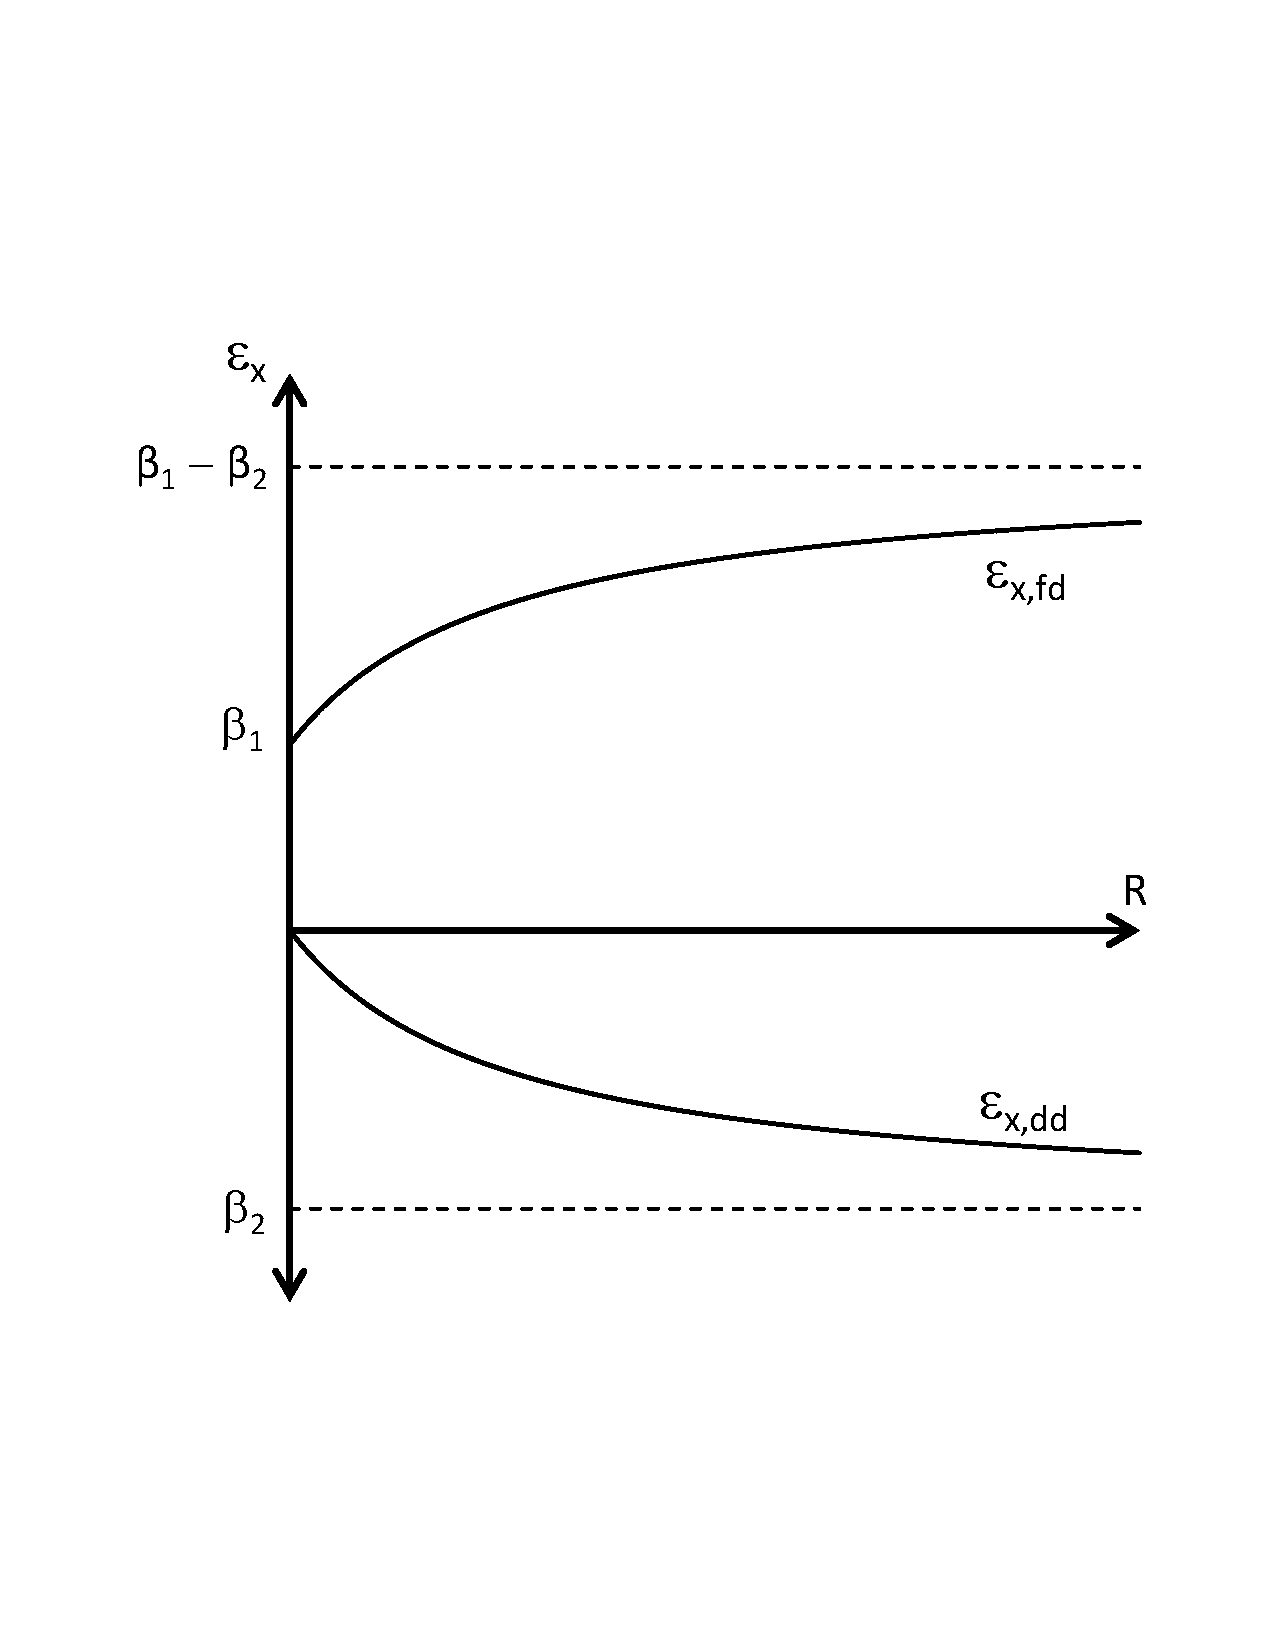
\includegraphics[trim={2cm 5cm 2cm 5cm},clip,width=0.5\linewidth]{figures/figure.pdf}
	\caption{Exports elasticities}
	\label{fig:elasticities}
\end{figure}


Intuitively, in the case of $\varepsilon_{x,dd}$, a percentage decrease in domestic sales that ends up being reoriented to the export market, will translate into a large (small) elasticity, in absolute terms, if domestic sales are large (small) in relative terms. Naturally, if there are no domestic sales, then no reorientation is possible and the elasticity is zero. In the case of $\varepsilon_{x,fd}$, if there are no domestic sales, the elasticity is given by $\beta_{1}$. As the domestic market gets more important, there is scope for reorientation, and the elasticity is higher.



\vspace{0.5cm}
(...)
\vspace{0.5cm}


%%%%%%%%%%%%%%%%%%%%%%%%%%


\section{Empirical results}\label{sec:results}

\subsection{Main results}\label{sec:results:main}

The estimations are reported in Table \ref{tb:regression}. The design of the different specifications and estimators is the following. First, we estimate the `traditional' log-linear model by fixed-effects, column `$ln\left (X_{it} \right )$ (FE)'. The dependent variable is the natural log of firms' exports. We assume the fixed-effects procedure is able to tackle all endogeneity issues associated with this specification.
Second, following the discussion in \cite{silva2006log} and in \cite{egger2015panel}, we account for heteroskedasticity and implement a (pseudo-maximum-likelihood) fixed-effects Poisson estimator. The dependent variable is now firms' exports (in levels), as described in equation (\ref{equation estimated}). The results are shown under column `$X_{it}$ (FE Poisson)'.


%%\begin{landscape}

\begin{table}[ht]
\caption{Determinants of firms' exports: FE \& Poisson}
\label{tb:regression}
\centering
\resizebox{1.0\textwidth}{!}
{\def\sym#1{\ifmmode^{#1}\else\(^{#1}\)\fi}
\begin{tabular}{lcc|cc|cc}
\hline\hline
\\[-1em]
 & \multicolumn{2}{c}{\small Panel A} & \multicolumn{2}{c}{\small Panel B} & \multicolumn{2}{c}{\small Panel C}\\[0.1cm] \hline
 &\multicolumn{1}{c}{$ ln(X_{it}) $ (FE)}&\multicolumn{1}{c|}{$ X_{it} $ (FE Poisson)}&\multicolumn{1}{c}{$ ln(X_{it}) $ (FE)}&\multicolumn{1}{c|}{$ X_{it} $ (FE Poisson)}&\multicolumn{1}{c}{$ ln(X_{it}) $ (FE)}&\multicolumn{1}{c}{$ X_{it} $ (FE Poisson)}\\[0.1cm]
\hline
 $ ln(FD_{it}) $&       0.477\sym{***}&       0.386\sym{***}&       0.406\sym{***}&       0.349\sym{***}&       0.416\sym{***}&       0.304\sym{***}\\[0.1cm]
            &     (0.011)         &     (0.043)         &     (0.013)         &     (0.040)         &     (0.020)         &     (0.044)         \\
 $ ln\left ( 1+\frac{DS_{i,t-1}}{X_{i,t-1}} \right )$&      -0.137\sym{***}&      -0.237\sym{***}&      -0.125\sym{***}&      -0.183\sym{***}&      -0.256\sym{***}&      -0.277\sym{***}\\
          &     (0.024)         &     (0.045)         &     (0.013)         &     (0.040)         &     (0.027)         &     (0.057)         \\
\hline
$ R^{2} $ within  &        0.50         &                     &        0.37         &                     &        0.46         &                     \\
Log-likelihood&            & -5436254         &            & -4544774         &             & -2455400         \\[0.1cm] \hline\hline
\multicolumn{7}{p{22.1cm}}{Notes.
The dependent variable $ln\left (X_{it} \right )$ denotes the (natural) log of exports for firm \textit{i} in period \textit{t}. $ln(FD_{it})$ stands for the log of Foreign Demand; $DS$ stands for Domestic Sales. FE corresponds to the linear fixed-effects estimator; FE Poisson reports fixed-effects Poisson estimates. The fixed-effects are at the firm level.
Robust standard-errors in parenthesis (clustered by firm). Significance levels: 1\%, ***; 5\%, **; 10\%, *.
All models include time dummies (which are jointly statistically significant in all estimations).
The models are estimated for three samples, panels A, B and C, respectively. Panel A corresponds to the full sample. In Panel B we drop observations if ratio $<$ 0.01 or $>$ 100, while in Panel C we drop observations if ratio $<$ 0.01 or $>$ 100 and keep just the firms that are in all periods.
The first sample has 21,749 observations, corresponding to 3,996 firms. The second sample uses 19,381 observations and 3,655 firms, while the third sample has 8,784 observations and 1,098 firms.
See Section \ref{sec:statistics} for a description of the data and Section \ref{sec:est:strategy} for a discussion on the estimation strategy.
\textit{Source}: Own computations.}
\end{tabular}}
\end{table}


\begin{figure}[ht]
	\centering
	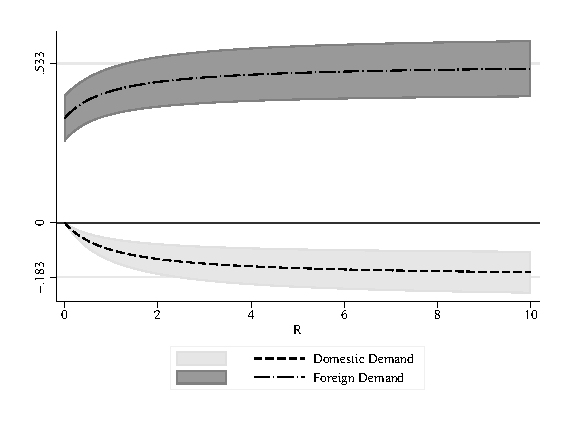
\includegraphics[width=0.7\linewidth]{figures/elasticities_estimated.eps}
	\caption{Estimated exports elasticities}
	\label{fig:elasticities:estimated}
\end{figure}


\begin{figure}[ht]
	\centering
	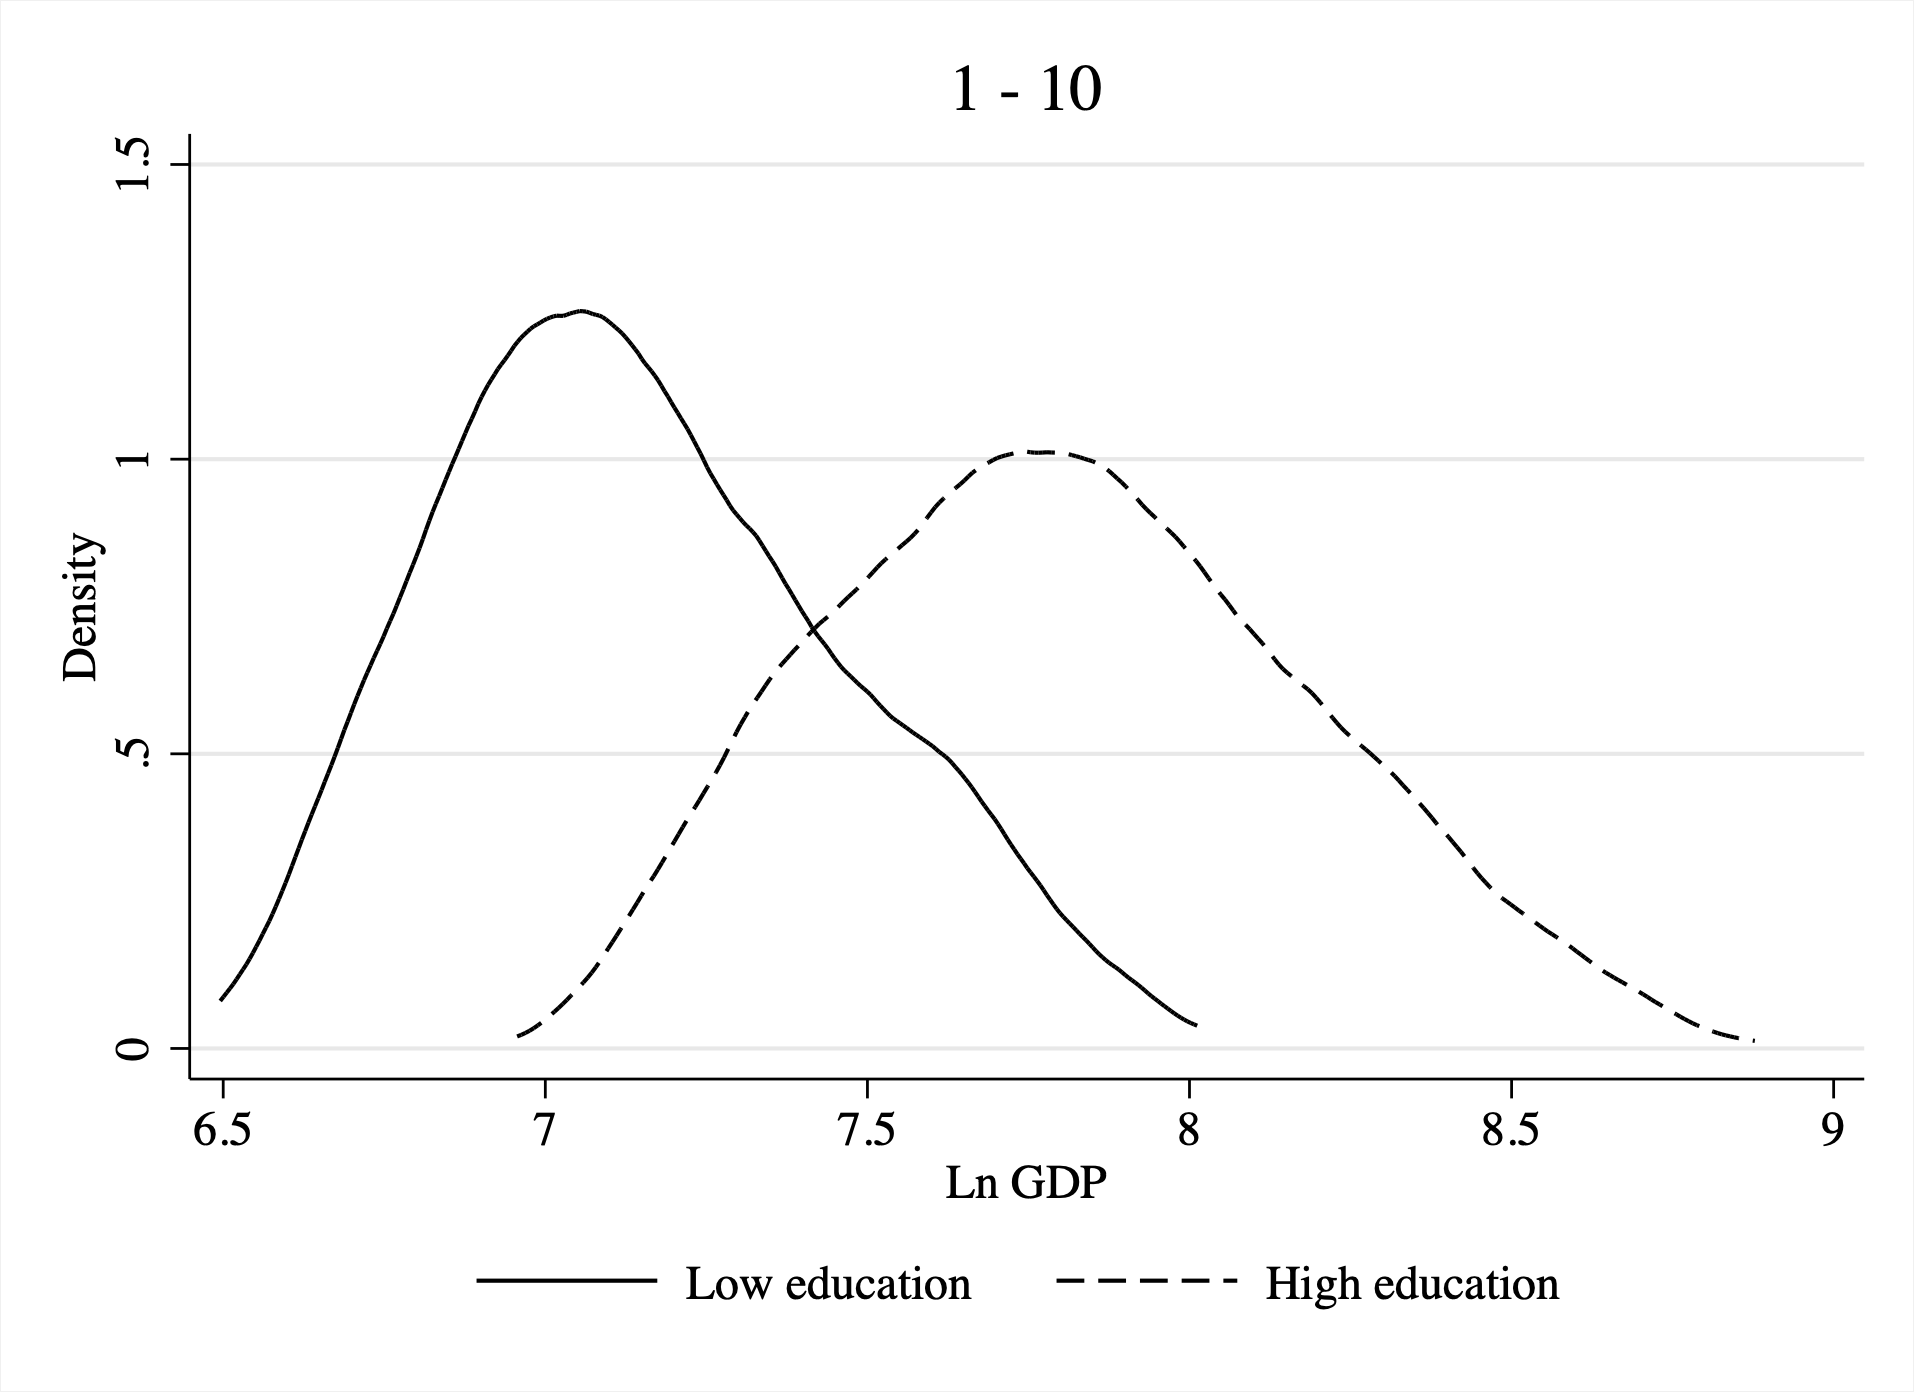
\includegraphics[width=0.7\linewidth]{figures/lnwage_education.png}
	\caption{Wages vs. Education}
	\label{fig:lnwage:education}
\end{figure}

\begin{comment}
\afterpage{%
\begin{table}[ht]
\caption{Estimation results} 
\label{tb:regressions}
\centering
\resizebox{0.8\textwidth}{!}
{\begin{tabular}{lccccc}
\noalign{\smallskip}\hline \noalign{\smallskip}
	\input{tables/estimations_paper_main_gmm_clean.tex}
\noalign{\smallskip}\hline \noalign{\smallskip}
\multicolumn{6}{p{15.7cm}}{\textit{Notes:} The dependent variable is $ln(GDP_{pc})_{i,t}$. All models are estimated by System--GMM (all models include as control variables $ln(Investment)_{i,t-1}$ and $ln(\Delta Employment)_{i,t}$ -- see equation (\ref{eq:growth})). Robust standard-errors in parenthesis and clustered at NUTS III level. Significance levels: 1\%, ***; 5\%, **; 10\%, *. Sample size:  184 observations, 23 NUTS III and 8 time periods.
AR(1) and AR(2) stand for the Arellano-Bond tests for first and second order autocorrelation in the first differences of the idiosyncratic disturbance term, $\Delta \varepsilon_{i,t}$; $pv$ stands for \textit{p-value}, while $df$ is degrees of freedom. Hansen refers to the test for joint validity of the instruments.
Descriptive statistics are reported in Table \ref{tb:statistics}. See the discussion in the main text for further information.}
\end{tabular}}
\end{table}
}
\end{comment}

\begin{table}
	\begin{center}
\begin{tabular}{lccccccc}
\hline \noalign{\smallskip} & OLS & RE & FE & IV & FE_IV & RE_IV & FE_cluster\\
\noalign{\smallskip}\hline \noalign{\smallskip}Education & 0.1072*** & 0.0666*** & 0.0624*** & 0.0551*** &  & 0.0563*** & 0.0624***\\
 & \begin{footnotesize}(0.0010)\end{footnotesize} & \begin{footnotesize}(0.0009)\end{footnotesize} & \begin{footnotesize}(0.0010)\end{footnotesize} & \begin{footnotesize}(0.0166)\end{footnotesize} & \begin{footnotesize}\end{footnotesize} & \begin{footnotesize}(0.0094)\end{footnotesize} & \begin{footnotesize}(0.0010)\end{footnotesize}\\
\noalign{\smallskip}Exper & 0.0131*** & 0.0045** & 0.0253*** & 0.0150 & 0.0562*** & 0.0045** & 0.0253***\\
 & \begin{footnotesize}(0.0022)\end{footnotesize} & \begin{footnotesize}(0.0019)\end{footnotesize} & \begin{footnotesize}(0.0008)\end{footnotesize} & \begin{footnotesize}(0.0092)\end{footnotesize} & \begin{footnotesize}(0.0009)\end{footnotesize} & \begin{footnotesize}(0.0018)\end{footnotesize} & \begin{footnotesize}(0.0008)\end{footnotesize}\\
\noalign{\smallskip}Exper2 & -0.0003*** & 0.0000 & 0.0000 & -0.0006 & -0.0000 & -0.0000 & 0.0000\\
 & \begin{footnotesize}(0.0001)\end{footnotesize} & \begin{footnotesize}(0.0000)\end{footnotesize} & \begin{footnotesize}(0.0000)\end{footnotesize} & \begin{footnotesize}(0.0005)\end{footnotesize} & \begin{footnotesize}(0.0000)\end{footnotesize} & \begin{footnotesize}(0.0000)\end{footnotesize} & \begin{footnotesize}(0.0000)\end{footnotesize}\\
\noalign{\smallskip}$R^2$ & 0.75 & . & 0.94 & 0.52 & . & . & 0.94\\
RMSE & 0.24 & 0.05 & 0.05 & 0.30 & . & . & 0.04\\
$N$ & 4,950 & 4,950 & 4,950 & 495 & 4,950 & 4,950 & 4,950\\
\noalign{\smallskip}\hline\end{tabular}\\
\smallskip\begin{footnotesize}\ * $p<0$.1; ** $p<0$.05; *** $p<0$.01\end{footnotesize}\\
\smallskip
\end{center}

\end{table}

\begin{table}[ht]
\caption{Regression analysis}\label{tb:regresults}
	\begin{center}
		\begin{center}
\begin{tabular}{lccccccc}
\hline \noalign{\smallskip} & OLS & RE & FE & IV & FE_IV & RE_IV & FE_cluster\\
\noalign{\smallskip}\hline \noalign{\smallskip}Education & 0.1072*** & 0.0666*** & 0.0624*** & 0.0551*** &  & 0.0563*** & 0.0624***\\
 & \begin{footnotesize}(0.0010)\end{footnotesize} & \begin{footnotesize}(0.0009)\end{footnotesize} & \begin{footnotesize}(0.0010)\end{footnotesize} & \begin{footnotesize}(0.0166)\end{footnotesize} & \begin{footnotesize}\end{footnotesize} & \begin{footnotesize}(0.0094)\end{footnotesize} & \begin{footnotesize}(0.0010)\end{footnotesize}\\
\noalign{\smallskip}Exper & 0.0131*** & 0.0045** & 0.0253*** & 0.0150 & 0.0562*** & 0.0045** & 0.0253***\\
 & \begin{footnotesize}(0.0022)\end{footnotesize} & \begin{footnotesize}(0.0019)\end{footnotesize} & \begin{footnotesize}(0.0008)\end{footnotesize} & \begin{footnotesize}(0.0092)\end{footnotesize} & \begin{footnotesize}(0.0009)\end{footnotesize} & \begin{footnotesize}(0.0018)\end{footnotesize} & \begin{footnotesize}(0.0008)\end{footnotesize}\\
\noalign{\smallskip}Exper2 & -0.0003*** & 0.0000 & 0.0000 & -0.0006 & -0.0000 & -0.0000 & 0.0000\\
 & \begin{footnotesize}(0.0001)\end{footnotesize} & \begin{footnotesize}(0.0000)\end{footnotesize} & \begin{footnotesize}(0.0000)\end{footnotesize} & \begin{footnotesize}(0.0005)\end{footnotesize} & \begin{footnotesize}(0.0000)\end{footnotesize} & \begin{footnotesize}(0.0000)\end{footnotesize} & \begin{footnotesize}(0.0000)\end{footnotesize}\\
\noalign{\smallskip}$R^2$ & 0.75 & . & 0.94 & 0.52 & . & . & 0.94\\
RMSE & 0.24 & 0.05 & 0.05 & 0.30 & . & . & 0.04\\
$N$ & 4,950 & 4,950 & 4,950 & 495 & 4,950 & 4,950 & 4,950\\
\noalign{\smallskip}\hline\end{tabular}\\
\smallskip\begin{footnotesize}\ * $p<0$.1; ** $p<0$.05; *** $p<0$.01\end{footnotesize}\\
\smallskip
\end{center}

	\end{center}
\end{table}


\vspace{0.5cm}
(...)
\vspace{0.5cm}



%%%%%%%%%%%%%%%%%%%%%%%%%%%%%%%%%%%%%%%%%%%%%%%%%%%%%%

\subsection{Robustness analysis}\label{sec:robust}
Beyond the analysis conducted above, two additional robustness checks are made to check if the results are affected by endogeneity and autocorrelation issues.


\vspace{0.5cm}
(...)
\vspace{0.5cm}



%%%%%%%%%%%%%%%%%%%%%%%%%%%%%%%%%%%%%%%%%%%%%%%%%%%%%%

\section{Heterogeneity across industries and firm size}\label{sec:results:industries}

There are reasons to believe that the link between domestic demand and exports could be different across firms. 

	\vspace{0.5cm}
	(...)
	\vspace{0.5cm}


%%%%%%%%%%%%%%%%%%%%%%%%%%%%%%%%%%%%%%%%%%%%%%%%%%%%%%

\section{Concluding remarks}\label{sec:conclusion}

The link between exports and domestic sales has been fuelling recent economic literature and the policy debate. In particular, the presence of a negative relationship may constitute an additional economic adjustment channel, in particular in the Euro area countries, where a common currency in a low inflation environment leads to the rigidity of real exchange rates.


	\vspace{0.5cm}
	(...)
	\vspace{0.5cm}

      

%%%%%%%%%%%%%%%%%%%%%%%%%%%%%%%%%%%%%%%%%%%%%%%%%%%%%%


\nocite{wooldridge1999distribution}
\nocite{vannoorenberghe2012firm}
\nocite{melitz2003impact}
\nocite{krugman1980scale}
\nocite{altomonte2013firm}

%%%%%%%%%%%%%%%%%%%%%%%%%%%%%%%%%%%%%%%%%%%%%%%%%%%%%%

\bibliography{references}

\end{document}
